\subsection{ETH measurements with block mining period 0s.}

\textit{Author: Jacek Janczura} \\
The measurements from the previous experiment were repeated with a new genesis. In new setup we decided to mine the block on demand. In that case demand is a presence of a transaction that is expected to be added to the blockchain. Using that method multiple transactions still might be fitting in a block but the miner is not wasting its mining power to mine empty blocks. This setup looks more like BASE or ACID database where transactions are executed immediately. 

\begin{table}[!h]
\centering
\begin{tabular}{l|l|l|}
\hline
\multicolumn{1}{|l|}{\textbf{tx}} & \textbf{tbn-t0 {[}s{]}} & \textbf{Thr. {[}tx/s{]}} \\ \hline
\multicolumn{1}{|l|}{\textit{10}} & \textit{0.08} & \textit{128.21} \\ \hline
\multicolumn{1}{|l|}{\textit{100}} & \textit{0.94} & \textit{105.93} \\ \hline
\multicolumn{1}{|l|}{\textit{1000}} & \textit{9.21} & \textit{108.59} \\ \hline
\multicolumn{1}{|l|}{\textit{10000}} & \textit{90.84} & \textit{110.09} \\ \hline
\multicolumn{1}{|l|}{\textit{100000}} & \textit{924.48} & \textit{108.17} \\ \hline
 & \textbf{AVG} & \textit{\textbf{112.20}} \\ \cline{2-3} 
\end{tabular}
\caption{ETH: Throughput measurement results. Mine on demand}
\label{table:3}
\end{table}

In Table \ref{table:3} we present the results of this new approach. In this case we are measuring throughput as total number of transactions divided by time from submitting the first transaction until mining the last block. Since the block frequency is not fixed we cannot measure the throughput using the method with block frequency - 2.1. Average throughput in that setup has raised to in average 112,2 transactions per second with an 1,02 average number of transactions per block 

\begin{figure}[!h]
    \centering
    %\captionsetup{justification=centering}
    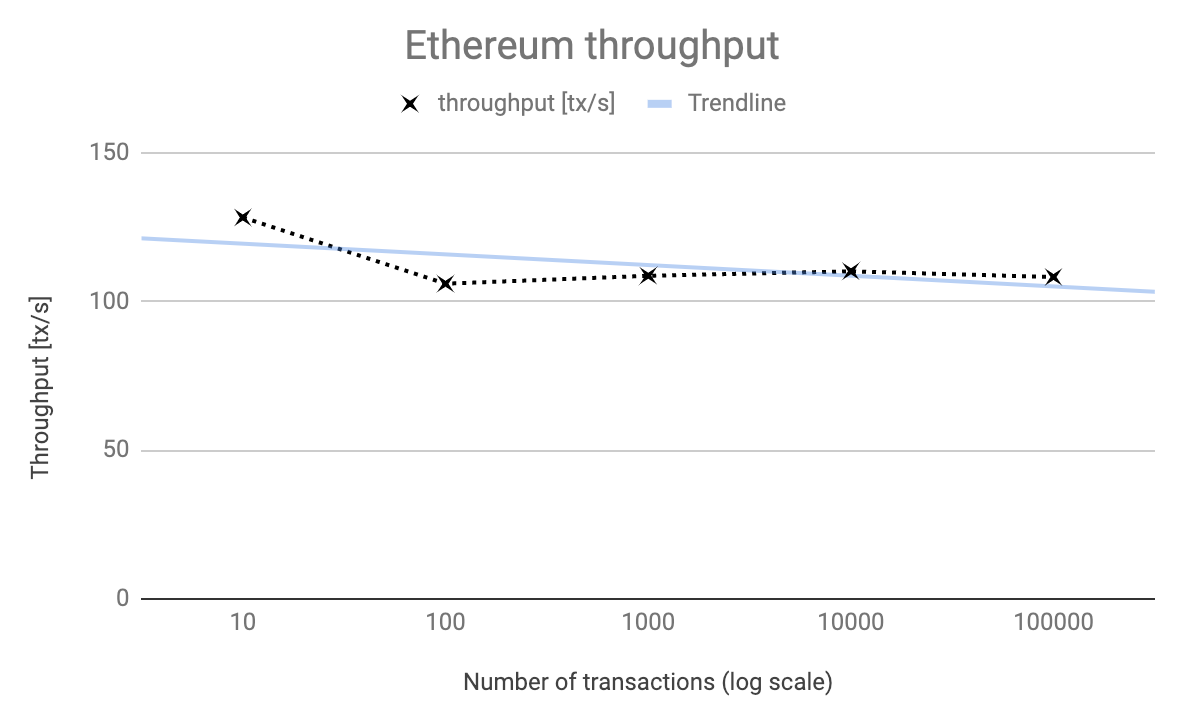
\includegraphics[width=0.75\textwidth]{img/Throughput0s.png}
   \caption{ETH: throughput on a log scale}
   \label{fig:tx0s}
\end{figure}

In this setup in Fig. \ref{fig:tx0s} we present the graph where we correlate the throughput with a number of transactions on a log scale. The throughput in that scenario is transaction independent and is in average around 100 tx/s.

Fig. \ref{fig:cap} depicts block capacity. This experiment was held on a milion transactions. It's clearly visible that in that setup miner submits on average 1 transaction per block and that value is stable within the whole experiment.

\begin{figure}[!h]
    \centering
    %\captionsetup{justification=centering}
    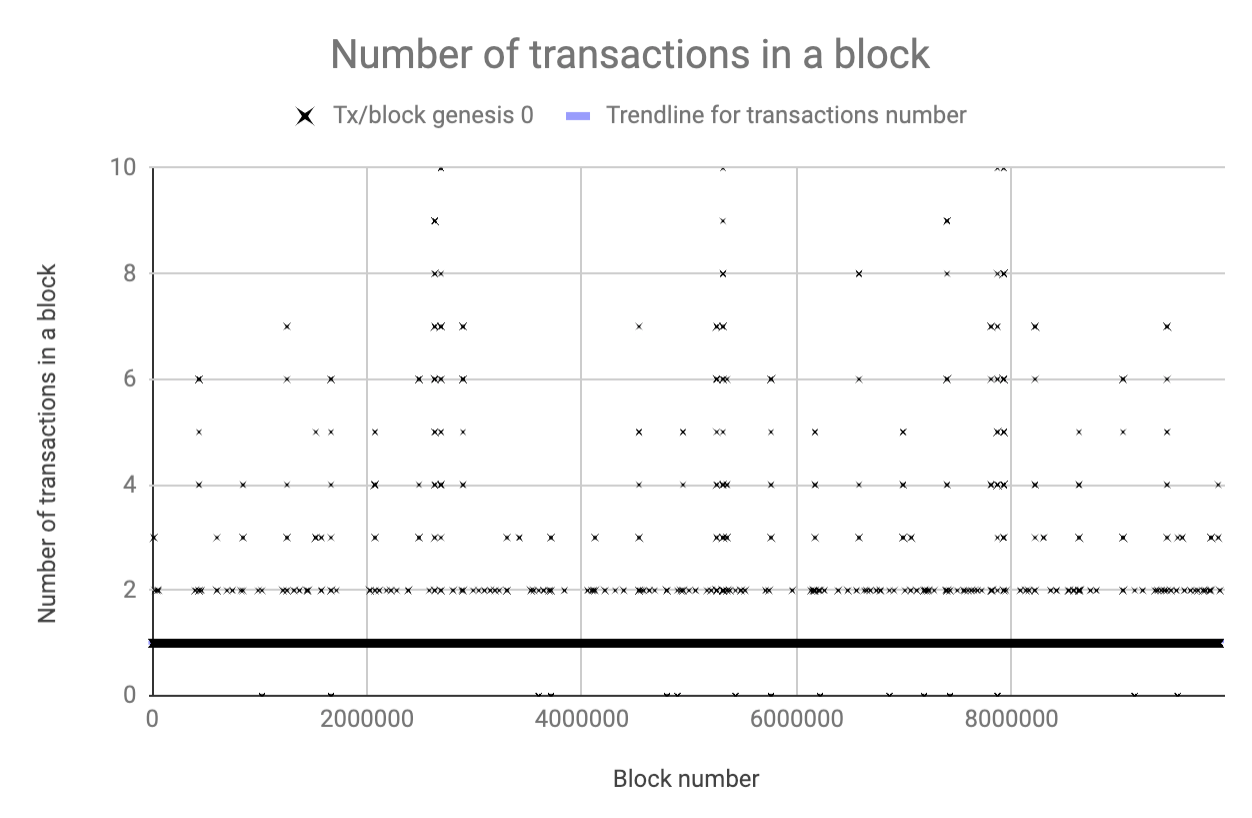
\includegraphics[width=0.75\textwidth]{img/blockCap0s.png}
   \caption{ETH: Block capacity}
   \label{fig:cap}
\end{figure}